
\subsection*{task 2.2 \\[1ex] Kronecker products for (na\"ive) upsampling}

The Kronecker product of an ordered pair of matrices (or 2D \emph{numpy} arrays) $\mat{A}, \mat{B}$ of sizes $k \times l $ and $m \times n$ respectively is defined as
\begin{equation*}
\mat{C} = \mat{A} \otimes \mat{B}
=
\begin{bmatrix}
a_{11} \mat{B} & a_{12} \mat{B} & \cdots & a_{1l} \mat{B} \\
a_{21} \mat{B} & a_{22} \mat{B} & \cdots & a_{2l} \mat{B} \\
\vdots & \vdots & \ddots & \vdots \\
a_{k1} \mat{B} & a_{k2} \mat{B} & \cdots & a_{kl} \mat{B} \\
\end{bmatrix}
\end{equation*}
and therefore produces a matrix (or 2D array) $\mat{C}$ of size $k \cdot m \times l \cdot n$.

Conveniently, \emph{numpy} provides the function \keyword{np.kron()} for the computation of Kronecker products. This allows us to realize a rather simple idea for \emph{upsampling} a small (intensity) image: assuming that the given image is stored in an array $\mat{F}$, we may simply compute
\begin{equation*}
\mat{G} = \mat{F} \otimes \mat{O}
\end{equation*}
where $\mat{O}$ denotes an $m \times n$ array of all ones.

Now, without using \keyword{for} loops, implement an appropriately parameterized function \keyword{upsample}. Then, load image \texttt{portrait.png} into \texttt{arrF} and compute
\begin{python}[emph={downsample,upsample}]
arrG = upsample(downsample(arrF, m, n), m, n)
\end{python}



\vspace{1cm}
Choose $(m,n) \in \bigl\{ (2,2), (4,4) \bigr\}$ and enter your results here (the figure already shows how your result should look like for $m=n=8$) 
%%%%%
%%%%%
%%%%% enter your result here, i.e. replace "placeholder.pdf" by the names of your resulting image files
%%%%%
%%%%%
\begin{figure}[h!]
\subfloat[$m = n = 1$]{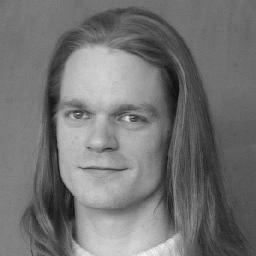
\includegraphics[width=0.24\textwidth]{portrait.png}} \hfill
\subfloat[$m = n = 2$]{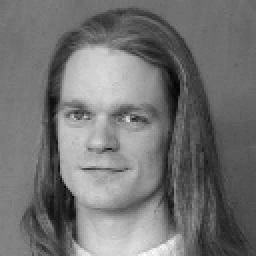
\includegraphics[width=0.24\textwidth]{t2-2.png}} \hfill
\subfloat[$m = n = 4$]{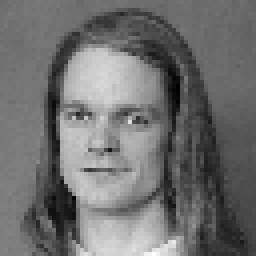
\includegraphics[width=0.24\textwidth]{t2-4.png}} \hfill
\subfloat[$m = n = 8$]{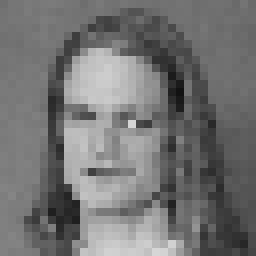
\includegraphics[width=0.24\textwidth]{t2-2-8x8.png}}
\end{figure}
%%%%%
%%%%%
%%%%%
%%%%%
%%%%%






